\documentclass[svgnames]{beamer}

\usepackage{pri}

\graphicspath{{./}{figures/}{figures/07-evaluation-figs/}} 

\subtitle{Evaluation of IR and IE Systems}


\begin{document}

\maketitle

\begin{frame} \frametitle{Bibliography}

   \begin{block}{}

        \href{http://www.cs.uic.edu/~liub/WebMiningBook.html}{Bing Liu, Web Data Mining: Exploring Hyperlinks, Contents, and
         Usage Data, 2nd edition}.  Chapter 6.  
    
    \end{block}

   \begin{block}{}

    \href{http://www.mir2ed.org/}{Ricardo Baeza-Yates,
            Berthier Ribeiro-Neto, Modern Information Retrieval, 2nd
            edtion}. Chapter 4.

    \end{block}

   \begin{block}{}

    \href{http://nlp.stanford.edu/IR-book/}{Christopher D. Manning, Prabhakar Raghavan and Hinrich Schütze, Introduction to Information Retrieval.} Chapter 8.

    \end{block}
    
\end{frame}



\section{Evaluation and Relevance}

\begin{frame} \frametitle{IR System Evaluation}
  
  \begin{block}{Why evaluate?}
      \begin{itemize}
      \item Measure the benefit of using an IR system
      \item Measure how well an IR system fulfills its goal
      \item Compare IR systems
      \end{itemize}

  \end{block}

  \begin{block}{What to evaluate?}
      \begin{itemize}
      \item Collection coverage
      \item Processing time
      \item Output presentation
      \item User effort
      \item \emph{Recall and Precision}
      \end{itemize}
  \end{block}

\end{frame}


% ----------------------------------------------------------------------

\begin{frame}
  \frametitle{Elements of an information retrieval performance evaluation experiment}

\begin{block}{The Cranfield Paradigm}

An IR experiment, as devised by Cyril Cleverdon (1950s), must include:

\begin{enumerate}

\item A reference collection
\item Relevance judgments
\item An evaluation metric

\end{enumerate}

\end{block}


\end{frame}

% ----------------------------------------------------------------------

\begin{frame}  \frametitle{Relevant Documents}
  
  \begin{block}{Recall and Precision} 
    Measure the ability of a system to return \emph{relevant} documents.
  \end{block}
  
  \begin{block}{Relevance}
    \begin{itemize}
    \item Subjective notion
    \item Usually \emph{evaluated by a set of experts}
    \end{itemize}
  \end{block}
\end{frame}

% ----------------------------------------------------------------------

\section{Precision vs. Recall}


\begin{frame}
  \frametitle{Evaluating Prediction}

  \begin{center}
    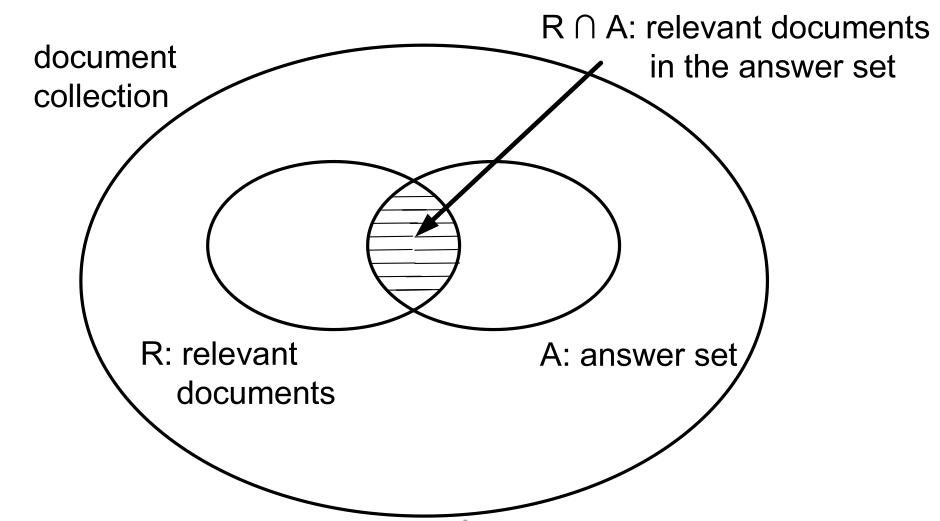
\includegraphics[width=1.0 \textwidth]{precision-recall}
  \end{center}
\end{frame}




\begin{frame}
  \frametitle{Measuring Precision and Recall}
  
  \begin{definition}
    Let $A$ be the set of documents retrieved for query $Q$. \\ 
    % A is the answer-set
    Let $R$ be the set of documents that are relevant to query $Q$.\\
    \emph{Precision} is the proportion of retrieved documents that are
    relevant, i.e.:
    \begin{displaymath}
      Pr = \frac{|R \cap A|}{|A|}
    \end{displaymath}
    \emph{Recall} is the proportion of relevant documents retrieved, i.e.:
    \begin{displaymath}
      Re = \frac{|R \cap A|}{|R|}
    \end{displaymath}
  \end{definition}
\end{frame}

% ----------------------------------------------------------------------

\begin{frame}
  \frametitle{Precision-Recall Curves}
  
  \begin{block}{}
    \begin{itemize}
    \item Retrieved documents are ordered $\Rightarrow$ we are interested in
      measuring how precision changes as recall increases
    \end{itemize}
  \end{block}

  \begin{example}
    Let $A = \{d_1, d_2, d_3, d_4, d_5, d_6, d_7, d_8, d_9, d_{10}\}$ be an
    ordered set of retrieved documents, for a query $Q$. 

    Let $R = \{d_2, d_5,d_8, d_{15}\}$ be the set of relevant documents for query $Q$.
    \begin{center}
      \begin{tabular}{c|c}
        $Re$ & $Pr$ \\\hline
        $0.25$ & $0.50$ \\
        $0.50$ & $0.40$ \\
        $0.75$ & $0.38$ \\
      \end{tabular}
    \end{center}
  \end{example}
\end{frame}

% ----------------------------------------------------------------------

\begin{frame}
  \frametitle{Interpolated Precision-Recall}
  
  \begin{block}{}
    \begin{itemize}
    \item Precision is usually measured at 10 standard recall points: $0\%,
      10\%, 20\%, ..., 90\%, 100\%$
    \item Precision at $r\%$ recall is defined as
      \begin{displaymath}
        P(r) = \max_{i \geq r}P(i)
      \end{displaymath}
    \item Precision is zero after no more relevant documents are found
    \end{itemize}
  \end{block}
\end{frame}

% ----------------------------------------------------------------------

\begin{frame}
  \frametitle{Interpolated Precision-Recall (cont.)}
  
%  \begin{example}
    Let $A = \{d_1, d_2, d_3, d_4, d_5, d_6, d_7, d_8, d_9, d_{10}\}$ be an
    ordered set of retrieved documents, for a query $Q$. Let $R = \{d_2, d_5,
    d_8, d_{15}\}$ be the set of relevant documents for query $Q$.
    
    \vspace{-4ex}

    \begin{columns}
      \column{0.2\linewidth}

      \begin{center}
          \small
          \begin{tabular}{c|c}
            $Re$ & $Pr$ \\\hline
            $0.25$ & $0.50$ \\
            $0.50$ & $0.40$ \\
            $0.75$ & $0.38$ \\
          \end{tabular}
      \end{center}

      \column{0.3\linewidth}

      \begin{center}
        \begin{tabular}{c|c}
          $Re$ & $Pr$ \\\hline
          $0.00$ & $0.50$ \\
          $0.10$ & $0.50$ \\
          $0.20$ & $0.50$ \\
          $0.30$ & $0.40$ \\
          $0.40$ & $0.40$ \\
          $0.50$ & $0.40$ \\
          $0.60$ & $0.38$ \\
          $0.70$ & $0.38$ \\
          $0.80$ & $0.00$ \\
          $0.90$ & $0.00$ \\
          $1.00$ & $0.00$
        \end{tabular}
      \end{center}

      \column{0.6\linewidth}
 
%      \resizebox{\linewidth}{!}{%GNUPLOT: LaTeX picture with Postscript
\begin{picture}(0,0)%
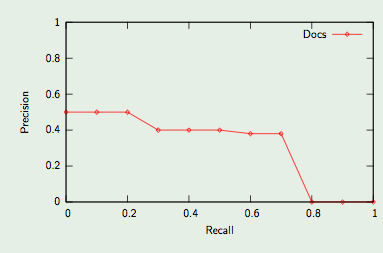
\includegraphics{pr}%
\end{picture}%
\begingroup
\setlength{\unitlength}{0.0200bp}%
\begin{picture}(18000,10800)(0,0)%
\put(2200,1650){\makebox(0,0)[r]{\strut{} 0}}%
\put(2200,3370){\makebox(0,0)[r]{\strut{} 0.2}}%
\put(2200,5090){\makebox(0,0)[r]{\strut{} 0.4}}%
\put(2200,6810){\makebox(0,0)[r]{\strut{} 0.6}}%
\put(2200,8530){\makebox(0,0)[r]{\strut{} 0.8}}%
\put(2200,10250){\makebox(0,0)[r]{\strut{} 1}}%
\put(2475,1100){\makebox(0,0){\strut{} 0}}%
\put(5415,1100){\makebox(0,0){\strut{} 0.2}}%
\put(8355,1100){\makebox(0,0){\strut{} 0.4}}%
\put(11295,1100){\makebox(0,0){\strut{} 0.6}}%
\put(14235,1100){\makebox(0,0){\strut{} 0.8}}%
\put(17175,1100){\makebox(0,0){\strut{} 1}}%
\put(550,5950){\rotatebox{90}{\makebox(0,0){\strut{}Precision}}}%
\put(9825,275){\makebox(0,0){\strut{}Recall}}%
\put(14950,9675){\makebox(0,0)[r]{\strut{}Docs}}%
\end{picture}%
\endgroup
\endinput
}
%      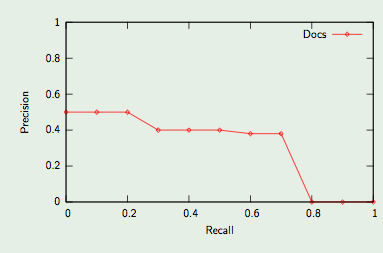
\includegraphics[width=\linewidth]{pr.eps}

          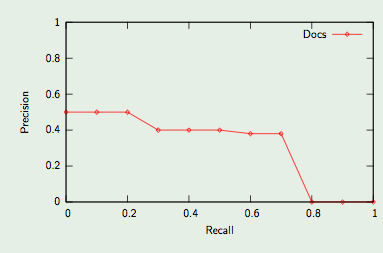
\includegraphics[width=.8\linewidth]{pr.png}\\

    \end{columns}
%  \end{example}
\end{frame}

% ----------------------------------------------------------------------

\begin{frame}
  \frametitle{Interpolated Precision-Recall (cont.)}
  
  \begin{example}
    \begin{center}
      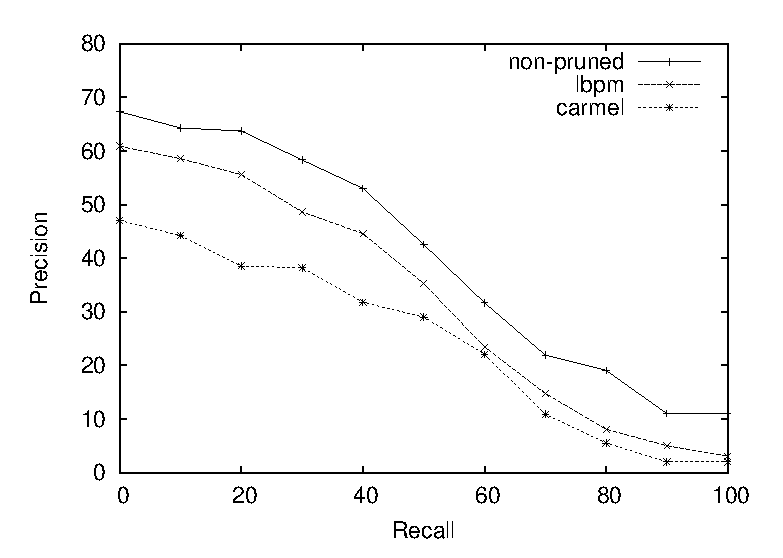
\includegraphics[width=0.8\linewidth]{size90.eps}
    \end{center}
  \end{example}
\end{frame}

% ----------------------------------------------------------------------

\section{Other Measures}

\begin{frame}
  \frametitle{P@$N$, R-precision }
  
  \begin{block}{P@$N$ -- Precision at the $N$-th retrieved document}
    Most commonly used 
  \begin{itemize}
    \item $P@5$, 
    \item $P@10$ 
    \item $P@20$
  \end{itemize}
  Usefull for Web retrieval
  \end{block}

  \begin{block}{}
\textbf{R-precision -} Precision at the $R$-th document, where $R$ is
      the number of relevant documents
  \end{block}

\end{frame}

\begin{frame}
  \frametitle{$F$-measure }
  \begin{block}{Harmonic mean of precision and recall:}
      \begin{displaymath}
        F_1 = \frac{2 \times Re \times Pr}{Re + Pr}
    \end{displaymath}
  \end{block}
\end{frame}





\begin{frame}
  \frametitle{AP, MAP}
  
  \begin{block}{}
    \begin{itemize}
    \item \textbf{AP -} Average of the values for the precision at each recall
        point
        \begin{displaymath}
            AP = \frac{\sum_{i=1}^N Pr@i \times R_i}{|R|}
        \end{displaymath}
        where $R_i = 1$ if document at rank $i$ is relevant and $R_i = 0$
        otherwise.
        % https://en.wikipedia.org/wiki/Information_retrieval#Mean_average_precision
    \item \textbf{MAP -} Mean Average Precision
        \begin{displaymath}
            \operatorname{MAP} = \frac{\sum_{q=1}^Q\operatorname{AP}_q}{Q}
        \end{displaymath}
    \item AP can also be interpolated
    \end{itemize}
  \end{block}
\end{frame}

\begin{frame}
  \frametitle{Discounted Cumulative Gain}
  
  \begin{block}{Cumulative gain: sum the relevance weights}
    \begin{itemize}
    \item \textbf{DCG -} Discounted cumulative gain
        \begin{displaymath}
            \operatorname{DCG}_p = R_1 + \sum_{i=2}^p\frac{R_i}{\log_2i}
        \end{displaymath}
        where $R_i = 1$ if document at rank $i$ is relevant and $R_i = 0$
        otherwise.
    \item \textbf{nDCG -} Normalized discounted cumulative gain
        \begin{displaymath}
            \operatorname{nDCG}_p = \frac{\operatorname{DCG_p}}{\text{Ideal}\operatorname{DCG}_p}
        \end{displaymath}
    \end{itemize}
  \end{block}
\end{frame}

\begin{frame}
  \frametitle{MRR}
  
  \begin{block}{MRR - Mean Reciprocal Rank}
        \begin{displaymath}
            \operatorname{MRR} = \frac{1}{N}\sum_{i=1}^N\frac{1}{\operatorname{rank}_i}
        \end{displaymath}
        where $\operatorname{rank}_1$ is the rank of the first relevant
        document.
  \end{block}
\end{frame}

\begin{frame} \frametitle{ERR}
\begin{block}{ERR - Expected Reciprocal Rank}
        \begin{eqnarray*}
            \operatorname{ERR} & = & \sum_{i=1}^N \frac{1}{N} \times {\operatorname{P}}(\text{user stops at position} i) \\
                               & = & \sum_{i=1}^N \frac{1}{N} \times \Pi_{i=1}^{N-1}(1 - R_i} R_N
        \end{eqnarray*}
        where $R_i = 1$ if document at rank $i$ is relevant and $R_i = 0$
  \end{block}
\end{frame}

\begin{frame}
    \frametitle{Ranking Comparison}

    \begin{block}{Spearman Coefficient}
        Computes the difference between the positions of a same document in two
        rankings
        \begin{displaymath}
            \rho(X,Y) = 1 - \frac{6\sum_{i=1}^N d_i^2}{N(N^2-1)}
        \end{displaymath}
        where $d_i = \operatorname{rank(X)}_i - \operatorname{rank(Y)}_i$ is
        the difference in rankings of document $i$.
        % https://en.wikipedia.org/wiki/Spearman%27s_rank_correlation_coefficient
    \end{block}

\end{frame}


\begin{frame}
    \frametitle{Ranking Comparison (cont.)}

    \begin{block}{Kendall's Tau}
        Let $(x_1, y_1), (x_2, y_2), \cdots, (x_N, y_N)$, where each $x_i$ is
        the rank of document $i$ in ranking $X$, and $y_i$ is the rank of
        document $i$ in ranking $Y$.
        \begin{displaymath}
            \tau = \frac{|\text{concordant pairs}| - |\text{discordant pairs}|}{N(N-1)/2}
        \end{displaymath}
        \small
        where a pair $(x_i, y_i)$ is concordant with $(x_j, y_j)$ if either:
        \begin{displaymath}
            \left\{
                  \begin{array}{l}
                    x_i > x_j \wedge y_i > y_j\\
                    x_i < x_j \wedge y_i < y_j
                  \end{array}
            \right.
        \end{displaymath}
        and discordant if either:
        \begin{displaymath}
            \left\{
                  \begin{array}{l}
                    x_i > x_j \wedge y_i < y_j\\
                    x_i < x_j \wedge y_i > y_j
                  \end{array}
            \right.
        \end{displaymath}
        % https://en.wikipedia.org/wiki/Kendall_rank_correlation_coefficient
    \end{block}

\end{frame}

% ------------------------------------------------------------

\section{Obtaining the Ground Truth}

\begin{frame}
  \frametitle{Reference Collections}

  \begin{block}{}
    \begin{description}
    \item[\href{http://trec.nist.gov/data.html}{TREC}] Various collections of
        documents (Ad hoc, Web, Blog, Clinical Decision Support, ...)
    \item[CACM] Articles from Communications of the ACM
    \item[ISI] Information science papers
    \item[CFC] Cystic Fibrosis Collection
    \item[...]
    \end{description}
  \end{block}

  \begin{block}{}
    \begin{itemize}
    \item Standards for research in IR
    \item Provide sets queries + evaluated documents
    \end{itemize}
  \end{block}
\end{frame}

% ------------------------------------------------------------

\begin{frame}
  \frametitle{Human Experimentation in the Lab}

\begin{itemize}
\item User preferences are affected by the characteristics of the user interface (UI)
\begin{itemize} 
\item For instance, the users of search engines look
  first at the upper left corner of the results page. 
\item Changing the layout is likely to affect the assessment
  made by the users and their behavior.
\end{itemize}
\item Proper evaluation of the user interface requires going beyond
  the framework of the Cranfield experiments
\end{itemize}


\end{frame}


\begin{frame}
  \frametitle{A/B Testing}

\begin{itemize}
\item A/B testing consists of displaying to selected users a modification in the layout of a page
\begin{itemize}
  \item The group of selected users constitute a fraction of all users such as, for instance, 1\%
  \item The method works well for sites with large audiences
\end{itemize}
\item By analysing how the users react to the change, it is possible to analyse if the modification proposed is positive or not
\end{itemize}

\begin{block}{} 
A/B testing provides a form of human experimentation, even if the setting is not that of a lab
\end{block}

\end{frame}


\begin{frame}
  \frametitle{Crowdsoursing}

\centering
\textbf{Amazon Mechanical Turk}
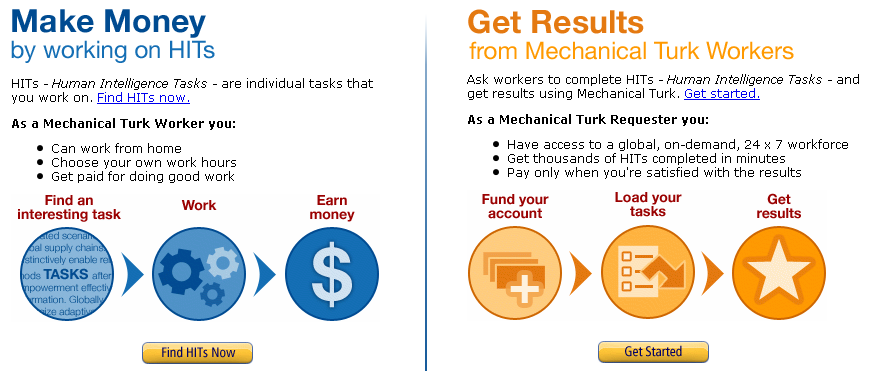
\includegraphics[width=0.8 \textwidth]{Amazon-Mechanical-Turk}\\
{\small \url{https://www.mturk.com}}

\begin{itemize}
    \small
\item The participants execute human intelligence tasks, called HITs, in exchange for small sums of money
\item The tasks are filed by requesters who have an evaluation need
\item While the identity of participants is not known to requesters,
  the service produces evaluation results of high quality (except for \emph{free-loaders, etc})
\end{itemize}

\end{frame}




\begin{frame}
  \frametitle{Evaluation using Clickthrough Data}

\begin{block}{A promising alternative...}
The data can be obtained by observing how frequently the users click on a given document, when it is shown in the answer set for a given query
\end{block}

%%This is particularly attractive because 
\begin{block}{Attractive, because...}
The data can be collected at a low cost without overhead for the use
\end{block}
\end{frame}


\section{Evaluation of Classifiers}

\begin{frame} \frametitle{Classifier Evaluation}
  
  \begin{itemize}
  \item Previous lectures have shown that tasks such as document classification or information extraction from text can be modeled as classification problems
  \begin{itemize}
  \item I.e., techniques in this section also apply to IE systems
  \end{itemize}  

  \item Goal in supervised classification is the minimization of classification error on test data
  
  \item We can evaluate through measures like recall, precision, and accuracy (i.e., one minus error)
  \begin{itemize}
  \item But classification tasks can involve more than two classes (i.e., more than distinguishing relevant from non-relevant)
  \end{itemize}  
  \end{itemize}

 \end{frame}

% % ------------------------------------------------------------

\begin{frame} \frametitle{Confusion Matrix}
  
 \begin{itemize}
 \item $M[i,j]$ is the number of test documents belonging to class $i$ which
     were assigned to class $j$
 \item Perfect classifier: diagonal elements $M[i,i]$ would be nonzero
 \item Example:
     \begin{displaymath}
         \footnotesize
         M = \left\{
             \begin{array}{c|c|c}
               5 & 0 & 0 \\\hline
               1 & 3 & 0 \\\hline
               1 & 2 & 4
             \end{array}
         \right\}
     \end{displaymath}
 \item If $M$ is large, we use
     \begin{displaymath}
         \text{accuracy} = \sum_i M[i,i] / \sum_{i,j} M[i,j]
     \end{displaymath}
 \item Notice that accuracy is not a good measure for {\it small} classes
 \end{itemize}

\end{frame}

% ------------------------------------------------------------

% \begin{frame} \frametitle{Multiple-class Scenario}
  
%  \begin{itemize}
%  \item One-vs.-rest
%    \begin{itemize}
%    \item Create a two-class problem for every class
%      \begin{itemize}
%      \item E.g. ``sports'' and ``not-sports'', ``science'' and
%        ``not-science'', etc.
%      \end{itemize}
%    \item We have a classifier for each case
%    \end{itemize}
%  \item Accuracy is measured by \emph{recall} and \emph{precision}
%    \begin{itemize}
%    \item Let $C_d$ be the correct classes for document $d$ and $C'_d$ be the
%      set of classes estimated by the classifier
%      \begin{displaymath}
%        precision = \frac{C'_d \cap C_d}{C'_d}
%      \end{displaymath}
%      \begin{displaymath}
%        recall = \frac{C'_d \cap C_d}{C_d}
%      \end{displaymath}
%    \end{itemize}
%  \end{itemize}
% \end{frame}

% % ------------------------------------------------------------

\begin{frame} \frametitle{Micro-Averaged Precision}
  
 In a problem with $n$ classes, let $C_i$ be the number of documents in class
 $i$ and let $C'_i$ be the number of documents estimated to be of class $i$ by
 the classifier
 \begin{itemize}
 \item \emph{Micro-averaged precision} is defined as
   \begin{displaymath}
     \frac{\sum_{i=1}^n C'_i \cap C_i}{\sum_{i=1}^n C'_i}
   \end{displaymath}
 \item \emph{Micro-averaged recall} is defined as
   \begin{displaymath}
     \frac{\sum_{i=1}^n C'_i \cap C_i}{\sum_{i=1}^n C_i}
   \end{displaymath}
 \end{itemize}

 \begin{itemize}
 \item Micro-averaged precision/recall measures correctly classified
   documents, thus favoring large classes
 \end{itemize}
\end{frame}

% ------------------------------------------------------------

\begin{frame} \frametitle{Macro-Averaged Precision}
  
 In a problem with $n$ classes, let $P_i$ and $R_i$ be the precision and
 recall, respectively, achieved by a classifier for class $i$
 \begin{itemize}
 \item \emph{Macro-averaged precision} is defined as
   \begin{displaymath}
     \frac{1}{n}\sum_{i=1}^n P_n
   \end{displaymath}
 \item \emph{Macro-averaged recall} is defined as
   \begin{displaymath}
     \frac{1}{n}\sum_{i=1}^n R_n
   \end{displaymath}
 \end{itemize}

 \begin{itemize}
 \item Macro-averaged precision/recall measures performance per class, giving
   all classes equal importance
 \end{itemize}
\end{frame}

% ------------------------------------------------------------

\begin{frame} \frametitle{$F_1$ measure}
  
    The \emph{$F_1$ measure} is also commonly used
    \begin{displaymath}
        F_1 = \frac{2 \times P_i \times R_i}{P_i + R_i}
    \end{displaymath}

    \begin{itemize}
    \item Harmonic mean between precision and recall
    \item Discourages classifiers that trade one for the other
    \end{itemize}

\end{frame}

% ------------------------------------------------------------


\finalframe{Questions?}

\end{document}
